\documentclass[12pt]{article}

%%%%%%%%%%%%%%%%%%%%%%%%%%%%%%%%%%%%%%%%%%%%%%%%%%%%%%%%%%%%%%%%%%%%%%%%%%%%%%%%%%%%%%%%%%%%%%%%%%%%
% Math
\usepackage{fancyhdr} 
\usepackage{amsfonts}
\usepackage{amsmath}
\usepackage{amssymb}
\usepackage{amsthm}
%\usepackage{dsfont}

%%%%%%%%%%%%%%%%%%%%%%%%%%%%%%%%%%%%%%%%%%%%%%%%%%%%%%%%%%%%%%%%%%%%%%%%%%%%%%%%%%%%%%%%%%%%%%%%%%%%
% Macros
\usepackage{calc}

%%%%%%%%%%%%%%%%%%%%%%%%%%%%%%%%%%%%%%%%%%%%%%%%%%%%%%%%%%%%%%%%%%%%%%%%%%%%%%%%%%%%%%%%%%%%%%%%%%%%
% Commands and Custom Variables	
\newcommand{\problem}[1]{\hspace{-4 ex} \large \textbf{Problem #1} }
\let\oldemptyset\emptyset
\let\emptyset\varnothing
\newcommand{\norm}[1]{\left\lVert#1\right\rVert}
\newcommand{\sint}{\text{s}\kern-5pt\int}
\newcommand{\powerset}{\mathcal{P}}
\renewenvironment{proof}{\hspace{-4 ex} \emph{Proof}:}{\qed}
\newcommand{\RR}{\mathbb{R}}
\newcommand{\NN}{\mathbb{N}}
\newcommand{\QQ}{\mathbb{Q}}
\newcommand{\ZZ}{\mathbb{Z}}
\newcommand{\CC}{\mathbb{C}}
\renewcommand{\Re}{\operatorname{Re}}
\renewcommand{\Im}{\operatorname{Im}}


%%%%%%%%%%%%%%%%%%%%%%%%%%%%%%%%%%%%%%%%%%%%%%%%%%%%%%%%%%%%%%%%%%%%%%%%%%%%%%%%%%%%%%%%%%%%%%%%%%%%
%page
\usepackage[margin=1in]{geometry}
\usepackage{setspace}
%\doublespacing
\allowdisplaybreaks
\pagestyle{fancy}
\fancyhf{}
\rhead{Shaw \space \thepage}
\setlength\parindent{0pt}

%%%%%%%%%%%%%%%%%%%%%%%%%%%%%%%%%%%%%%%%%%%%%%%%%%%%%%%%%%%%%%%%%%%%%%%%%%%%%%%%%%%%%%%%%%%%%%%%%%%%
%Code
\usepackage{listings}
\usepackage{courier}
\lstset{
	language=Python,
	showstringspaces=false,
	formfeed=newpage,
	tabsize=4,
	commentstyle=\itshape,
	basicstyle=\ttfamily,
}

%%%%%%%%%%%%%%%%%%%%%%%%%%%%%%%%%%%%%%%%%%%%%%%%%%%%%%%%%%%%%%%%%%%%%%%%%%%%%%%%%%%%%%%%%%%%%%%%%%%%
%Images
\usepackage{graphicx}
\graphicspath{ {images/} }
\usepackage{float}

%tikz
\usepackage[utf8]{inputenc}
\usepackage{pgfplots}
\usepgfplotslibrary{groupplots}

%%%%%%%%%%%%%%%%%%%%%%%%%%%%%%%%%%%%%%%%%%%%%%%%%%%%%%%%%%%%%%%%%%%%%%%%%%%%%%%%%%%%%%%%%%%%%%%%%%%%
%Hyperlinks
%\usepackage{hyperref}
%\hypersetup{
%	colorlinks=true,
%	linkcolor=blue,
%	filecolor=magenta,      
%	urlcolor=cyan,
%}

\begin{document}
	\thispagestyle{empty}
	
	\begin{flushright}
		Sage Shaw \\
		m566 - Spring 2018 \\
		\today
	\end{flushright}
	
{\large \textbf{HW - Chapter 6}}\bigbreak

\problem{4 (a)} Given data $\{(t_i,z_1)\}_{i=0}^m$, the model $u(t) = \gamma_1 e^{\gamma_2 t}$ cannot be fit to said data using the techniques in this chapter, because the parameters are not linear combinations of functions of the data.

\bigbreak
\problem{4 (b)} Convert the model into a linear model and fit it to the data below.

\begin{center}
	\begin{tabular}{|c|c|c|c|}
		\hline
		$i$&1&2&3\\ \hline
		$t_i$&0.0&1.0&2.0\\ \hline
		$z_i$&$e^{0.1}$&$e^{0.9}$&$e^{2}$\\ \hline
	\end{tabular}
\end{center}

The model above can be rewritten as $\ln(u(t)) = \ln(\gamma_1) + \gamma_2 t$. Using this representation we can construct an overdetermined linear system.
$$
%L^{-1} = 
\begin{bmatrix}
1 & t_1\\
1 & t_2\\
1 & t_3
\end{bmatrix}
\begin{bmatrix}
ln(\gamma_1)\\
\gamma_2
\end{bmatrix}
=
\begin{bmatrix}
ln(z_1)\\
ln(z_2)\\
ln(z_3)
\end{bmatrix}
%= L^\prime
$$

Applying a least squared method we find that the parameters of best fit are $\gamma_1 = 1.0512711$ and $\gamma_2 = 1.0512711$. This exponential regression can be seen in the plot below along with our data. The code that generated these results can be found in the appendix.

\begin{figure}[H]
	\caption{Data points in green and the exponential regression in blue.}
	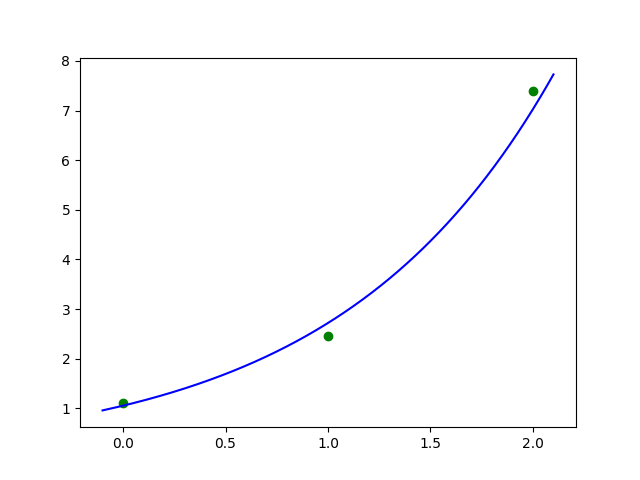
\includegraphics[width=.75\textwidth]{hw1_figure_1.png}
	\label{p1_T_err}
	\centering
\end{figure}

\problem{5 (a)} Suppose one generalized the LU decomposition to full rank matrices of size $m \times n$ for $m>n$. Since $m \ne n$ at least one of the matrices $L \in \RR^{m \times k}$ or $U\in \RR^{k \times n}$ must not be square. If $L$ is not square then the initial forward substitution will fail since the system is over determined. If $U$ is not square a similar situation arises in the back substitution. It should be noted that if $k<n$ then $\text{Rank}(LU) \le k < n$.

\bigbreak
\problem{5 (b)} \textbf{**************************}

\bigbreak
\problem{6 (a)} 

\begin{proof} First recall that if $A$ has full rank then $\text{Rank}(AB) = \text{Rank}(B)$. \bigbreak
	Note that $Q$ is orthogonal so $Q^{-1} = Q^T$ exists and $Q$ is full rank. Thus $\text{Rank}(A) = \text{Rank}(R)$. Since $R$ is upper triangular $\text{det}(R) = \prod\limits_{i=1}^n r_{ii}$. Thus $R$ is full rank (i.e. not singular) if and only if its diagonal entries are all non-zero. Thus $A$ has full column rank if and only if the diagonal entries of $R$ are all-non zero.
\end{proof}

\bigbreak
\problem{6 (b)} Since $I \in \RR^{n\times n}$ is non-singular, $\text{Rank}(Q) = n$. Thus $\text{Rank}(A) = \text{Rank}(R)$. The rest follows as in the previous proof.

\end{document}
